\documentclass{article}

\usepackage{amsmath}
\usepackage[utf8]{inputenc}
\usepackage{graphicx}
\usepackage{biblatex} 
\addbibresource{references.bib} %Import the bibliography file
\begin{document}

\title{\textbf{Fast Fourier Transform with MPI}}
\author{Ismail Kerem Tatlici (517418), Shubham Shubhankar Sharma (517420)}
\date{\today}
\maketitle
\section{Introduction}

This project discusses the parallelization of the Fast Fourier Transform (FFT)\cite{fft_wikipedia} algorithm using MPI (Message Passing Interface) for computing FFT in  2D. The project begins by presenting and describing the mathematical formulas for the 1D and 2D FFT algorithms. Next, the available parallelism in the FFT algorithm is studied, and different strategies for parallelization of the 2D FFT algorithm using MPI are discussed. Two approaches are presented, and the first approach, which involves dividing the data into smaller chunks and distributing them among different processes, is selected for the MPI implementation. The project also presents the theoretical assessment of strong and weak parallelism using the first approach. Finally, the project concludes by discussing the results of the MPI implementation of the 2D FFT algorithm.
\\\\
Our aim for this project was to implement FFT in 2D to show strong scalability and weak scalability on GCP using MPI for different sized images to achieve maximum speedup.

\section{Analysis of the serial algorithm}
\subsection{Fast Fourier Transform in 1D}
The one-dimensional Fast Fourier Transform (1D-FFT)\cite{fft_video} is a computational algorithm used to decompose a signal in the time or spatial domain into its corresponding frequency components in the frequency domain. The 1D-FFT is based on the mathematical concept of the discrete Fourier transform (DFT), which is a way of representing a finite sequence of data points in the complex plane. We used Cooley-Tukey algorithm\cite{cooley1965algorithm} for this purpose.
\\\\
The mathematical formula for the one-dimensional Fast Fourier Transform (FFT) of a sequence of $N$ complex numbers, $x_n$, is given by:

\begin{equation*}
X_k = \sum_{n=0}^{N-1} x_n \cdot W_N^{kn}, \quad \text{for } n = 0 \text{ to } N-1
\end{equation*}

where $X_k$ is the $k$-th output frequency component, $x_n$ is the $n$-th input sample, $W_N = e^{-j \cdot 2 \pi / N}$ is the $N$-th root of unity, and $k$ and $n$ are integer values that range from 0 to $N-1$.
\\\\
The inverse FFT (IFFT) is given by:

\begin{equation*}
x_n = \frac{1}{N} \sum_{k=0}^{N-1} X_k \cdot W_N^{-kn}, \quad \text{for } k = 0 \text{ to } N-1
\end{equation*}

\subsection{Fast Fourier Transform in 2D}

The two-dimensional Fast Fourier Transform (2D-FFT) is a computational method used to decompose an image or signal in the spatial domain into its corresponding frequency components in the frequency domain. It is an extension of the one-dimensional Fast Fourier Transform (1D-FFT) and is used to analyze images and other two-dimensional signals.
\\\\
The 2D-FFT algorithm works by first decomposing the image or signal into rows, and then for each row, it applies the 1D-FFT algorithm. The resulting frequency coefficients are then arranged in a two-dimensional matrix. Next, the algorithm transposes this matrix and decomposes each column using the 1D-FFT. The final result is a two-dimensional matrix of frequency coefficients that represents the original image or signal in the frequency domain.

\section{A-priori study of available parallelism.}
\subsection{Strategies for parallelisation for the MPI program of FFT 2D.}

\subsubsection{First Approach}

This approach involves dividing the data into smaller chunks and distributing them among the different processes:
\begin{enumerate}
\item First, the master divides the 2D input matrix $complex<double>[][]$ in a set of rows depending on the number of cores. For example: If we have a $512\times512$ matrix and 4 processes (1 master and 3 slaves), then each of the processes will get $(512\times512/4) = 128\times512$ sized matrix.

\item After that, the slave performs FFT 1D on the rows of the sub-matrix individually. This result is sent back to the master.

\item The sending and receiving of the sub-matrix is done through MPI\_Send and MPI\_Recv. As these are blocking functions, the processes will only start doing computation once the data has been received completely.

\item The master first combines all these results into a single matrix and then takes a transpose of the same.
All the steps will run for the second iteration. This time the FFT is done on the columns (because of the transpose).

\item  Finally all the slaves send the data back to the master which compiles it into the final matrix. This matrix is written into a txt file. 
\end{enumerate}

\subsubsection{Second Approach}

The 1D FFT can be parallelized to some extent using MPI, but it is limited by the nature of the FFT algorithm itself. The FFT algorithm relies on a divide-and-conquer approach, where the input signal is split into even and odd indices, and then each of these sub-signals is transformed separately. This process continues recursively until the size of the sub-signals becomes small enough to be transformed directly.
\\\\
In the 1D FFT, this divide-and-conquer approach results in a sequential process, where each step of the transformation depends on the result of the previous step. This makes it difficult to parallelize the 1D FFT using MPI, as each process would need to wait for the results from other processes before it can continue.


\subsection{A-priori theoretical assessment}

We are going to use the first approach for our MPI implementation. Here, the total execution time is computed using the following formula:
\begin{equation*}
        et = sct + pt
\end{equation*}
        where et = Total Execution Time,\\
        sct = Synchronization and Communication time between master and slave processes,\\
        pt = Actual processing of data by slave and master.

\subsubsection{Strong Parallelism (Fat Cluster):}

According to this approach, as we increase the number of cores for a fixed-sized image, our execution time should decrease linearly until a certain point and then become constant. For the fat cluster, we are going to use 2 machines in the same region with 16 cores each. So, \textit{sct} will be small as the distance between the master and slave processors are short. These are some of our expectations:

\begin{enumerate}
    \item The distance between master and slave processor is less if they are on the same virtual machine, and more if they are on different virtual machines. 
    \item As we increase the size of the image (e.g. 8192x8192), the speed up in comparison to a smaller sized image (e.g., 512x512) is much better with the increase in number of cores. This behavior could be explained by the fact that when the images are smaller, \textit{sct} dominates the \textit{pt}. But as we increase the size of the image, \textit{pt} starts dominating \textit{sct}.

\end{enumerate}

\subsubsection{Weak Parallelism (Intra Regional Light Cluster):}

According to this approach, as we increase the number of cores for a fixed-sized image, our execution time should decrease linearly until a certain point and then become constant. But in comparison to the fat cluster, the time taken would be more as the distances between the master processor and the slave processors are bigger.

For the intra-regional light cluster, we are going to use 16 machines in the same region with 2 cores each. So, \textit{sct} will be larger as the master and the slave processor are much further away. These are some of our expectations:

\begin{enumerate}
    \item In this case, there are 15 different slave machines. As we increase the size of the image (e.g. 8192x8192), the total execution time series for fat clusters and weak clusters shows more similar behavior. This is because the \textit{pt} starts dominating \textit{sct} as we increase the size of images. \item On the other hand, with smaller images (e.g. 2048x2048), \textit{sct} is larger in light clusters than the fat clusters, the \textit{pt} is always smaller in the fat cluster than the light cluster.

\end{enumerate}

\subsubsection{Weak Parallelism (Inter Regional Light Cluster):}

According to this approach, as we increase the number of cores for a fixed-sized image, our execution time should increase linearly. For the inter-regional light cluster, we are going to use 16 machines with 2 cores each. Out of the 16 machines, 2 will be in the same region (one master and slave), 14 will be divided in three regions (different from the region of the master). These are some of our expectations:

\begin{enumerate}
\item The linear increase could be attributed to the fact that \textit{sct} becomes so huge, that increasing the number of cores which decreases the \textit{pt} by dividing the task into smaller parts doesn’t help much.

\end{enumerate}

\subsection{Profiling}

We used \texttt{valgrind} as tools for profiling the serial and the parallel code.
The compilation of the binary was done with \texttt{-O2} optimization and with the \texttt{-g} flag.

\begin{verbatim}
g++ -g -O2 -o fft_serial.out fft_serial.cpp
\end{verbatim}

Command used for \texttt{valgrind}:

\begin{verbatim}
valgrind --tool=callgrind --main-stacksize=999999999 ./fft_serial 512
\end{verbatim}

\begin{table}[htbp]
\centering
\begin{tabular}{|c|c|c|c|}
\hline
Matrix Size & Number of Instructions & Time elapsed(sec) & CPI (2.2 Ghz) \\
\hline
512x512 & 3,815,937,072 & 0.833983 & 0.4808157381 \\
\hline
1024x1024 & 15,722,423,038 & 3.5549 & 0.4974284168 \\
\hline
2048x2048 & 64,874,945,375 & 15.1177 & 0.5126623199 \\
\hline
4096x4096 & 259,499,781,500 & 65.7212 & 0.557174419 \\
\hline
8192x8192 & 1,037,999,126,000 & 288.415 & 0.6112847151 \\
\hline
\end{tabular}
\caption{Serial Code}
\label{tab:serial}
\end{table}

\begin{table}[h]
\centering
\begin{tabular}{|c|c|c|c|}
\hline
Matrix Size & Number of Instructions & Time elapsed(sec) & CPI (2.2 Ghz) \\ 
\hline
512x512 & 3,815,937,072 & 0.439615 & 0.2534509825 \\ 
\hline
1024x1024 & 15,722,423,038 & 1.75092 & 0.2450019307 \\ 
\hline
2048x2048 & 64,874,945,375 & 7.22725 & 0.2450861409 \\ 
\hline
4096x4096 & 259,499,781,500 & 30.5155 & 0.2587058055 \\ 
\hline
8192x8192 & 1,037,999,126,000 & 116.396 & 0.2466969322 \\
\hline
\end{tabular}
\caption{MPI Code with 8 Cores}
\end{table}
\newpage
\begin{figure}[h]
    \centering
    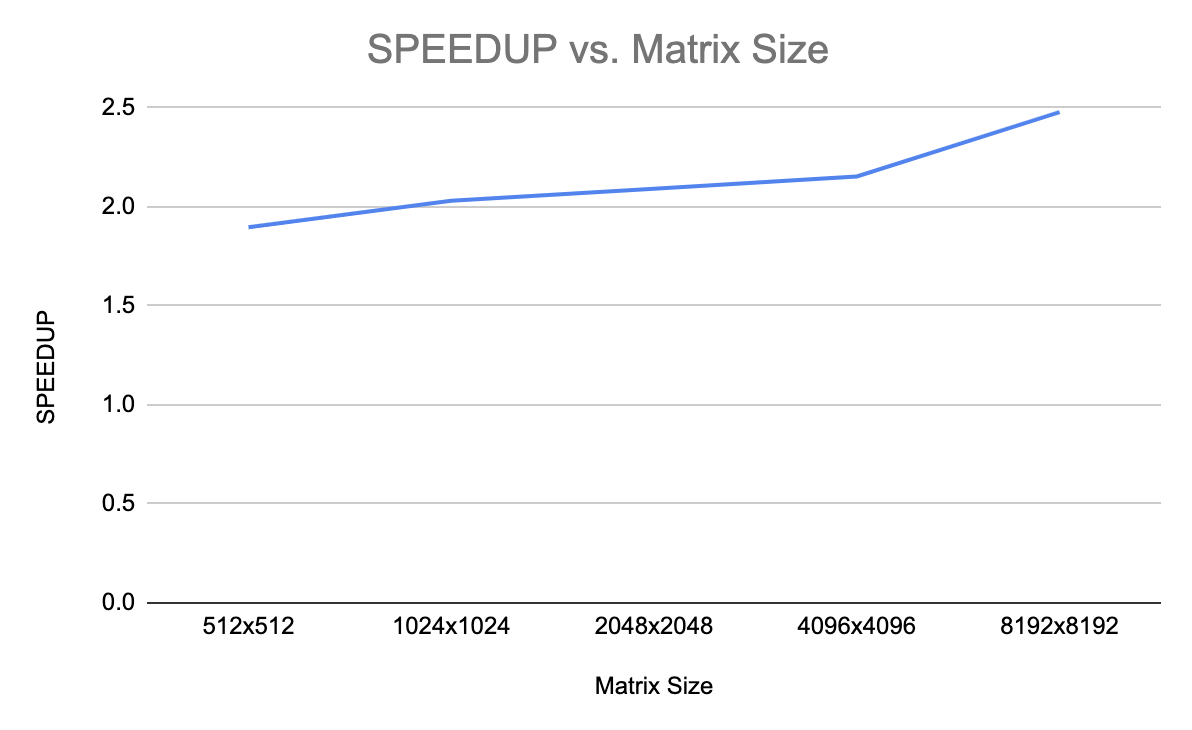
\includegraphics[width=400px]{Amdahlv1.png}
    \caption{ A-priori theoretical assessment using Amdahl's Law }
    \label{fig:Amdahl}
\end{figure}

\section{MPI parallel implementation.}
In this implementation, we have used MPI\_Send() and MPI\_Recv() to send the data of $complex<double>$ type from master to slave and vice-versa. The master divides the data and then sends it to the slave. The below figures illustrates this process in detail.

\begin{figure}[h]
    \centering
    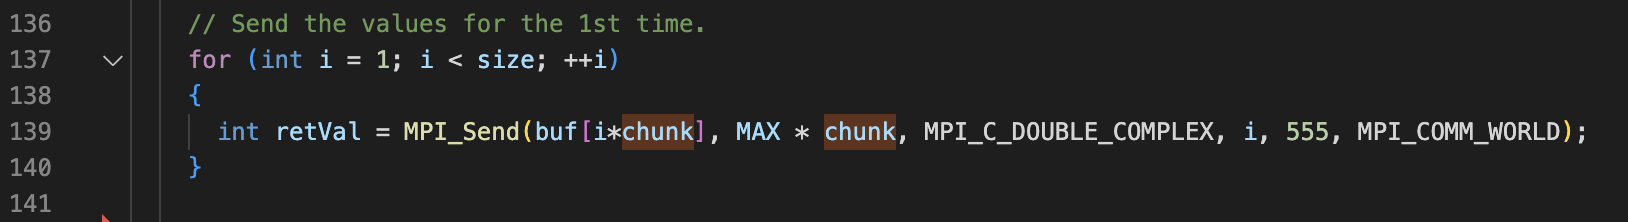
\includegraphics[width=400px]{mpisend1.png}
    \caption{Sending the data from master to slave}
    \label{fig:Sending}
\end{figure}

\begin{figure}[h]
    \centering
    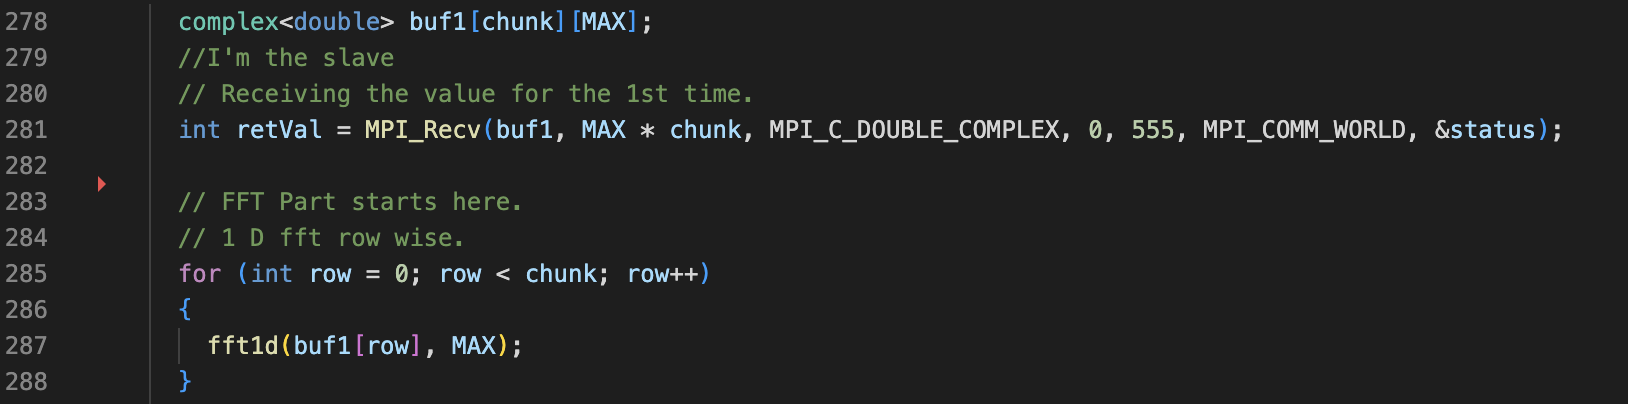
\includegraphics[width=400px]{mpirecv.png}
    \caption{Receiving the data from master to slave and implementing 1D-FFT on rows}
    \label{fig:Receiving}
\end{figure}
\newpage
\begin{enumerate}
    \item We adopted the first approach explained in section 2.1.1.
    \item The images read by the python program called "convert\_image.py" from "datasets/rgb/" folder and that python program converts the images into gray scale and save the images as a txt file into "datasets/gray/" folder.
    \item The image  is read from the "datasets/gray/" which are in text format. The image size is provided by the user and correspondingly an image in txt format is read from the folder. 
    \item The application applies FFT-2D and IFFT-2D and store the results in "results/fft\_txt"
    \item Than by running another python program which called read\_txt\_image.py, reads the result images from  "results/fft\_txt" file and convert them into png image files into "results/fft\_png" folder.
\end{enumerate}
\newpage
\section{GCP Implementation}
\subsection{Fat Cluster Setup}

\begin{figure}[h]
    \includegraphics[width=.90\textwidth]{fatcluster.png}
\\[\smallskipamount]
\\[\smallskipamount]
    
\includegraphics[width=.90\textwidth]{FatCluster.png}
\end{figure}
\newpage

\subsection{Intra Regional Cluster Setup}
\begin{figure}[h]
    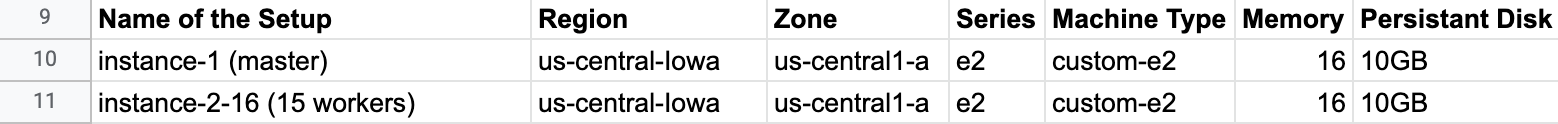
\includegraphics[width=.90\textwidth]{intra.png}
\\[\smallskipamount]
\\[\smallskipamount]
    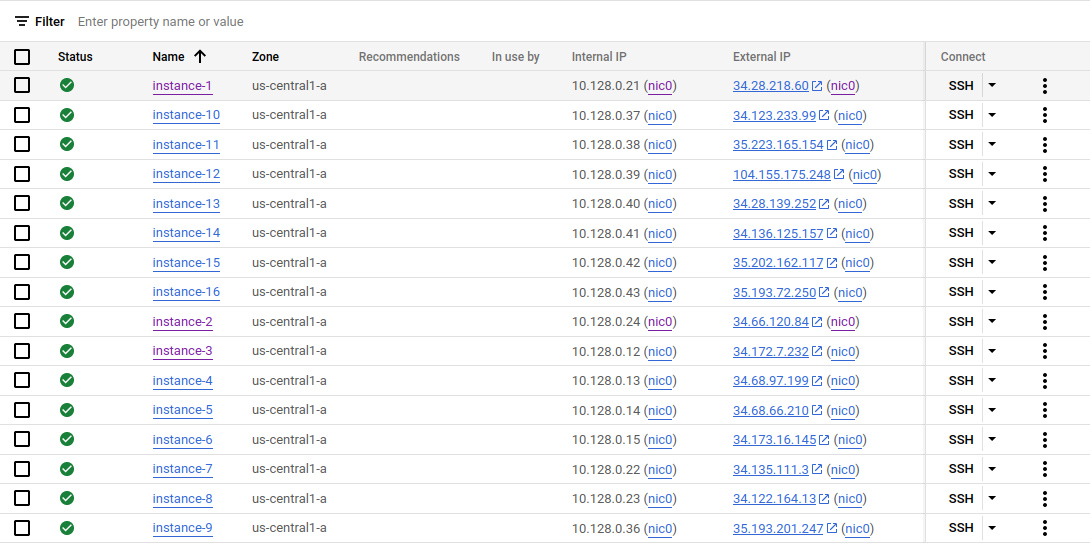
\includegraphics[width=.90\textwidth]{lightCluster.intraRegional.png}
\end{figure}

\subsection{Inter Regional Cluster Setup}
\begin{figure}[h]
    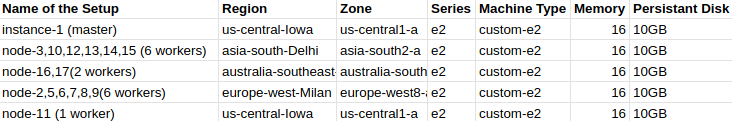
\includegraphics[width=.90\textwidth]{Setup Light Cluster (Inter Regional).png}
\\[\smallskipamount]
\\[\smallskipamount]
    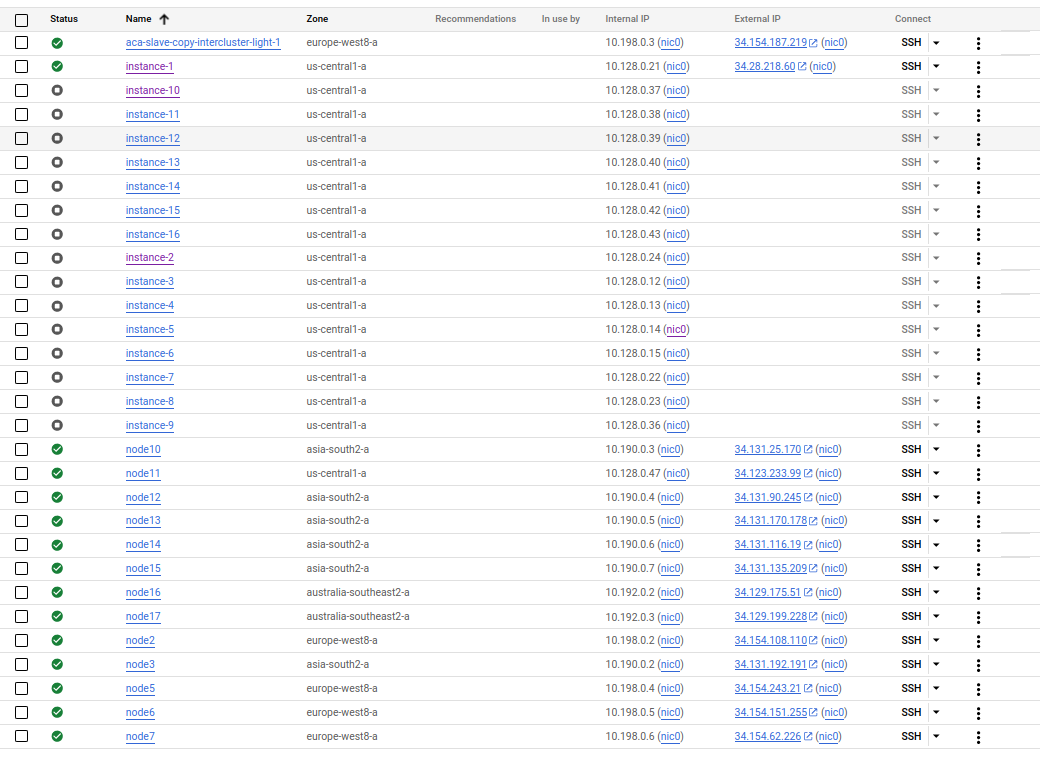
\includegraphics[width=.90\textwidth]{lightCluster.interRegional.png}
\end{figure}
\newpage
\section{Testing and Debugging}
\begin{enumerate}
    \item We were having issues with sizes bigger than 256x256. Because of the stack size we were having that issue and once we make our systems stack size unlimited with \texttt{ulimit -s unlimited} command our problem solved for the local machine.
    \item For the first time, when we create a new virtual machine, we have to manually establish a connection by ssh into the machine and then back to the source. This creates an entry in the known\_hosts file in \texttt{.ssh} folder. And the next time, when we try to connect. There are no issues of such kind. For example: If we have 15 slaves and 1 master. We have to go to these machines one by one from our master node and create this connection.
    \item The quota issues number with IN\_USE\_ADDRESSES (static IP range) region=us-central1 was increased from 24 to 48. 
    \item Connection time out error when deploying the inter-regional clusters. \item The quota issue number with CPUS (region=us-central1) and CPUS\_ALL\_REGIONS was increased from 24 to 96.
    \item In a single machine if we just run \texttt{fft\_mpi.cpp} it gives us proper results. But if we want to do this in a light cluster we had to increase the stack size permanently in each of the machines by copying this command at these three files:
    In file \texttt{/etc/security/limits.conf}. The below-given command increases the hard and soft limit for the stack for all users to unlimited.
    \begin{verbatim}
                hard stack unlimited
                soft stack unlimited
    \end{verbatim}
        In file \texttt{/etc/profile} and \texttt{/etc/bash.bashrc}, we added
    \begin{verbatim}
    ulimit -s unlimited
    \end{verbatim}
    \item When we tried to run our mpi code by using multiple virtual machines in GCP with the following command:
    \begin{verbatim}
    mpirun -np 4 --hostfile hostfile
    \end{verbatim}
    We got this error:
    \begin{verbatim}
        ORTE was unable to reliably start one or more daemons.
    \end{verbatim}
    In order to resolve this problem, we used \texttt{--prefix} parameter in the \texttt{mpirun} command, which is shown below:
    \begin{verbatim}
    mpirun --prefix /usr/local/openMPI/ -np 8 --hostfile hostfile fft_mpi
    \end{verbatim}
    \item When we open the ssh connection from GCP directly, it deletes the \texttt{authorized\_keys} inside the \texttt{.ssh} folder and replaces it with its own key. To counter this problem, we have added a line of code in \texttt{.bashrc}

\begin{verbatim}
(cat .ssh/id_rsa.pub >> .ssh/authorized_keys)
\end{verbatim}

in all our nodes. We only access GCP ssh for the master so this issue remains limited to the master only for the time being.

\end{enumerate}
\newpage
\section{Performance and Scalability Analysis}

\subsection{Execution Time:} The main purpose of parallelism is to reduce the execution time of a program. As a result of the experiment below charts were drawn for fat cluster, intra-regional  and inter-regional light clusters with their execution time for the 5 different sized images. It is seen that not all the parallel configurations achieved the purpose of parallelism. 

\begin{figure}[hb]
    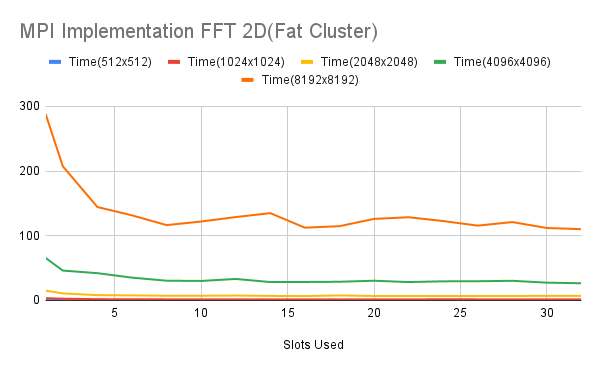
\includegraphics[width=.48\textwidth]{MPI Implementation FFT 2D(Fat Cluster).png}\hfill
    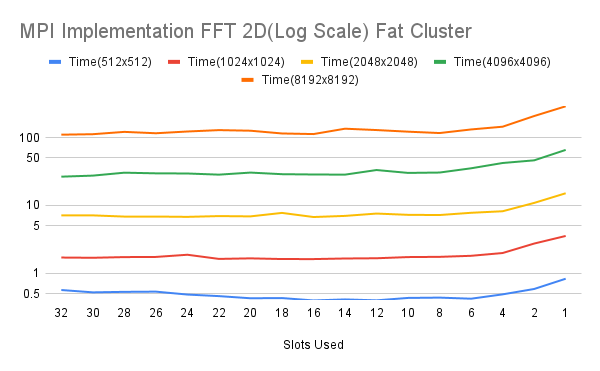
\includegraphics[width=.48\textwidth]{MPI Implementation FFT 2D(Log Scale) Fat Cluster.png}
    \\[\smallskipamount]
    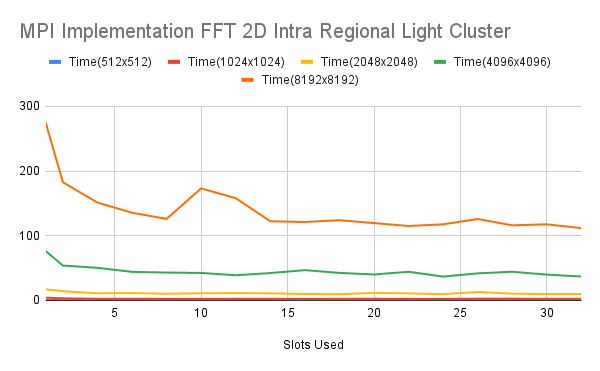
\includegraphics[width=.48\textwidth]{MPI Implementation FFT 2D Intra Regional Light Cluster.png}\hfill
    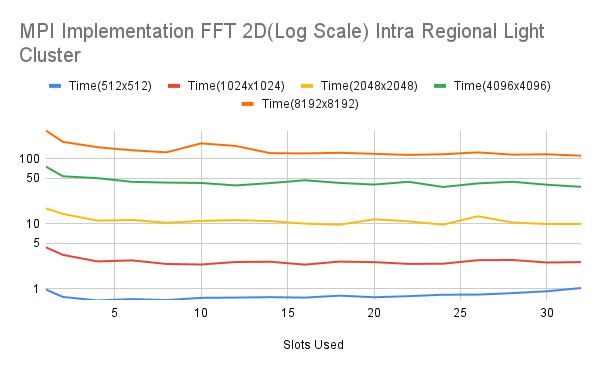
\includegraphics[width=.48\textwidth]{MPI Implementation FFT 2D(Log Scale) Intra Regional Light Cluster.png}
    \\[\smallskipamount]
    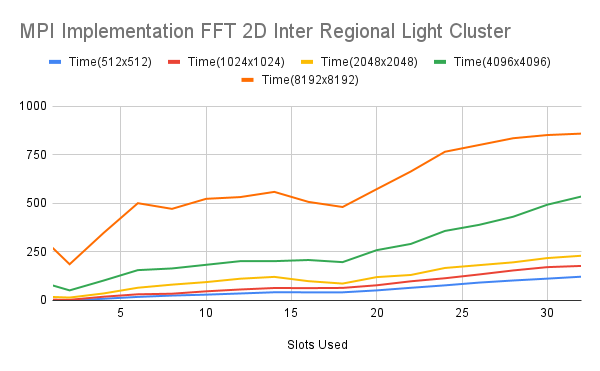
\includegraphics[width=.48\textwidth]{MPI Implementation FFT 2D Inter Regional Light Cluster.png}\hfill
    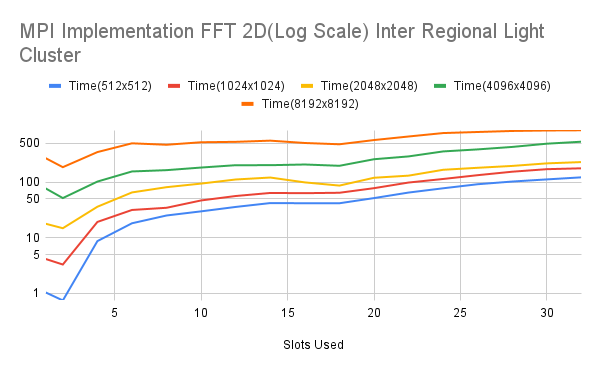
\includegraphics[width=.48\textwidth]{MPI Implementation FFT 2D(Log Scale) Inter Regional Light Cluster.png}
    \caption{Execution time comparision Fat Cluster vs Light Intra Regional Cluster vs Light Inter Regional Cluster}\label{fig:foobar}
\end{figure}
\newpage
\subsection{Number of Communications between Master and Slave}

\begin{tabular}{|c|c|c|c|}
\hline
No. of comm. & Slots & Master & Slave \\
\hline
4   & 2 & 1 & 1 \\
\hline
12  & 4 & 1 & 3 \\
\hline
20  & 6 & 1 & 5 \\
\hline
28  & 8 & 1 & 7 \\
\hline
36  & 10 & 1 & 9 \\
\hline
44  & 12 & 1 & 11 \\
\hline
52  & 14 & 1 & 13 \\
\hline
60  & 16 & 1 & 15 \\
\hline
68  & 18 & 1 & 17 \\
\hline
76  & 20 & 1 & 19 \\
\hline
84  & 22 & 1 & 21 \\
\hline
92  & 24 & 1 & 23 \\
\hline
100 & 26 & 1 & 25 \\
\hline
108 & 28 & 1 & 27 \\
\hline
116 & 30 & 1 & 29 \\
\hline
124 & 32 & 1 & 31 \\
\hline
\end{tabular}



\subsection{Memory Occupancy: }
\begin{verbatim}
8192x8192x16 = 2^31 = 2147.48365 megabytes
4096x4096x16 = 2^29 = 536.870912 megabytes
2048x2048x16 = 2^27 = 134.217728 megabytes
1024x1024x16 = 2^25 = 33.554432 megabytes
512x512x16   = 2^23 = 8.388608 megabytes    
\end{verbatim}

\subsection{Speed Up}
Using the figure 5, one can infer these things.
\subsubsection{Fat Cluster}
\begin{enumerate}
    \item As we increase the size of the image, the speedup increases while keeping the slot size constant.
    \item  As we increase the number of slots while keeping the image size constant, the speedup increases till a point(around 14 slots) and then becomes constant.
\end{enumerate}
\subsubsection{Light Cluster(Intra Regional)}
\begin{enumerate}
    \item As we increase the size of the image, the speedup increases while keeping the slot size constant.
    \item  As we increase the number of slots while keeping the image size constant, the speedup increases till a point(around 14 slots) and then becomes constant.
\end{enumerate}
\subsubsection{Light Cluster(Inter Regional)}
\begin{enumerate}
    \item As we increase the size of the image, the speedup increases while keeping the slot size constant.
    \item As we increase the number of slots while keeping the image size constant, the speedup decreases.
\end{enumerate}

\textbf{Note:} On comparing fat cluster and light cluster, the speedup in fat cluster is more than speedup in light cluster for the same sized image(e.g 4096x4096 image) as shown in below given figure.
\newpage
\begin{figure}[hb]
    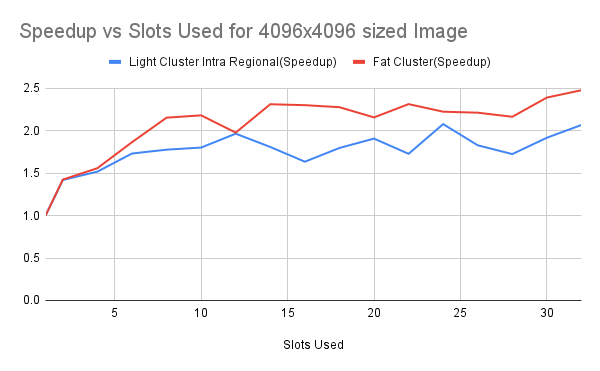
\includegraphics[width=.48\textwidth]{Speedup vs Slots Used for 4096x4096 sized Image.png}\hfill
    \label{Fast Cluster vs Light Cluster Speedup}
    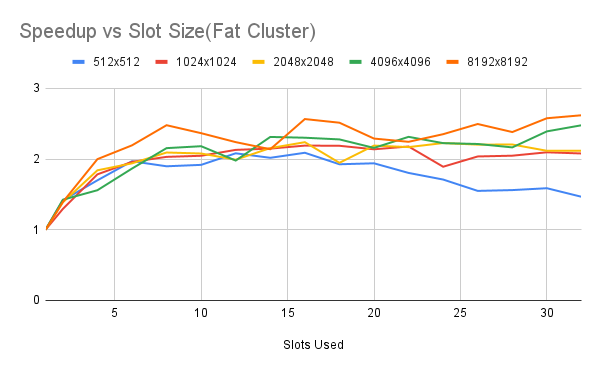
\includegraphics[width=.48\textwidth]{Speedup vs Slot Size(Fat Cluster).png}
    \\[\smallskipamount]
    \centering
    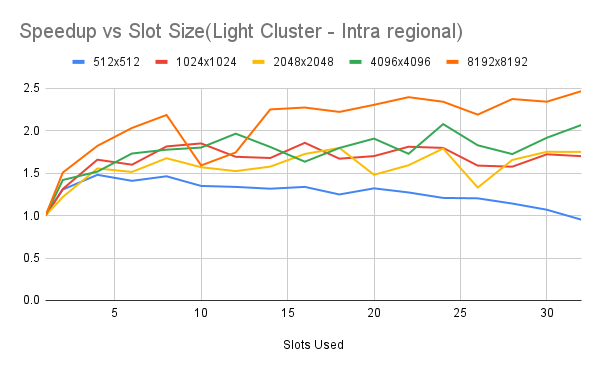
\includegraphics[width=.48\textwidth]{Speedup vs Slot Size(Light Cluster - Intra regional).png}\hfill
    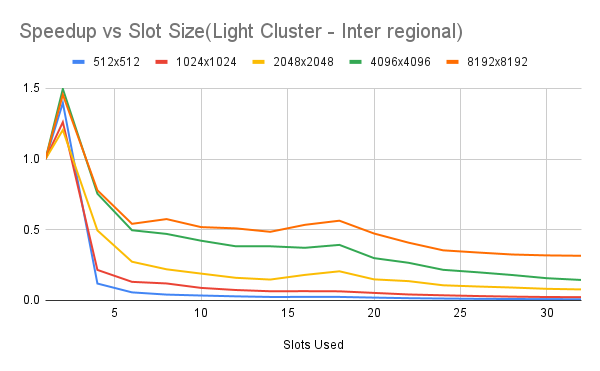
\includegraphics[width=.48\textwidth]{Speedup vs Slot Size(Light Cluster - Inter regional).png}
    \caption{Speedup comparision for different type of clusters.}
    \label{fig:Weak Scalability(Intra)}
\end{figure}
\newpage
\subsection{Strong Scalability} As per our hypothesis shown in the a-priori theoretical assessment, the execution time decreases as we increase the number of slots for a given fixed size image.(i.e 8192x8192). As predicted, when the number of slots reaches a certain point(14 and above in our case), the speedup becomes almost constant. This is due to an increase in MPI communication overhead. The increase in synchronization and communication time between the master and the slave process counters the faster execution done by each process on the sub-matrix.
\begin{figure}[hb]
    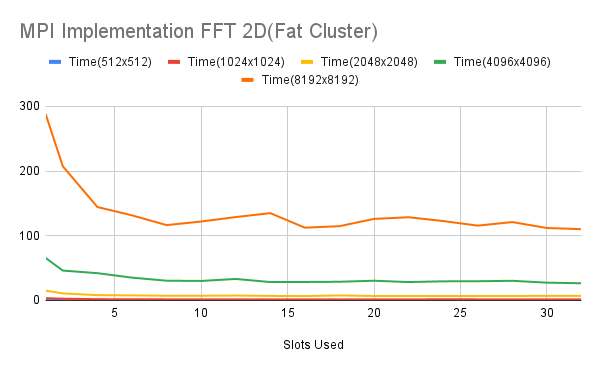
\includegraphics[width=.48\textwidth]{MPI Implementation FFT 2D(Fat Cluster).png}\hfill
    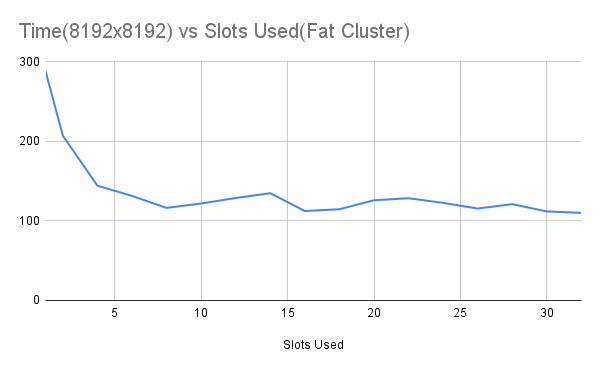
\includegraphics[width=.48\textwidth]{Time(8192x8192) vs Slots Used(Fat Cluster).png}
    \caption{Strong Scalability for different size of images}
    \label{fig:Strong Scalability}
\end{figure}
\newpage
\subsection{Weak Scalability}
\subsubsection{Intra-Regional Cluster}
As per our hypothesis shown in the a-priori theoretical assessment,
the execution time decreases as we increase the number of slots for a given fixed size image.(i.e 8192x8192). As predicted, when the number of slots reaches a certain point(14 and above in our case), the speedup becomes almost constant.
This behavior is similar to what we observe in strong scalability, but the communication overhead is more than the fat clusters  because the distance between the master and the slave process is larger.
\begin{figure}[hb]
    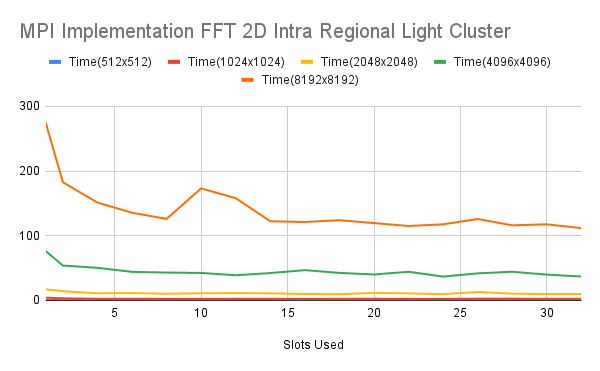
\includegraphics[width=.48\textwidth]{MPI Implementation FFT 2D Intra Regional Light Cluster.png}\hfill
    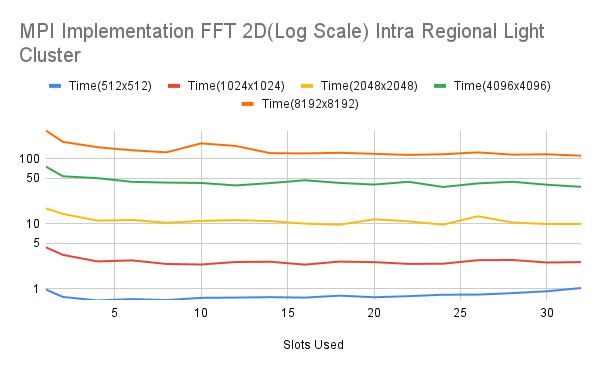
\includegraphics[width=.48\textwidth]{MPI Implementation FFT 2D(Log Scale) Intra Regional Light Cluster.png}
    \caption{Weak Scalability(Intra) for different size of images}
    \label{fig:Weak Scalability(Intra)}
\end{figure}

\subsubsection{Inter-Regional Cluster}
As per our hypothesis shown in the a-priori theoretical assessment, as we increase the number of cores for a fixed-sized image, our execution time should increase linearly.
The effect is more prominent in inter-regional clusters than the intra-regional clusters because in inter-regional clusters the communication overhead is humungous in comparison to intra-regional clusters.

\begin{figure}[hb]
    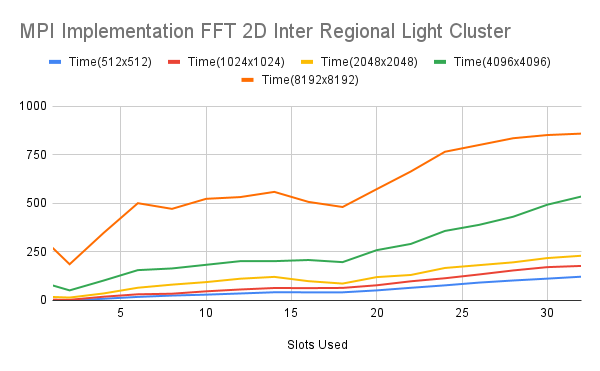
\includegraphics[width=.48\textwidth]{MPI Implementation FFT 2D Inter Regional Light Cluster.png}\hfill
    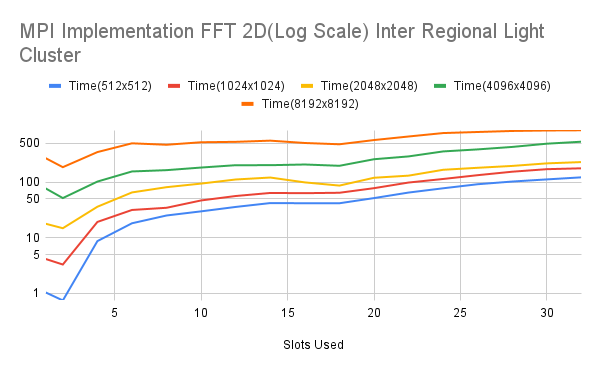
\includegraphics[width=.48\textwidth]{MPI Implementation FFT 2D(Log Scale) Inter Regional Light Cluster.png}
    \caption{Weak Scalability(Inter) for different size of images}
    \label{fig:Weak Scalability(Inter)}
\end{figure}
\newpage

\newpage

\section{Conclusion}

As parallel programming is mostly concerned about performance, a good project must also provide significant speedup.
\begin{enumerate}
    \item For the fat cluster, with 8192x8192 image, we are able to achieve a speedup of  2.62 with 32 slots. 
    \item As shown in Performance and Scalability Analysis, we are able to scale our program using mpi to achieve strong scalability with fat cluster.
    \item For the light cluster(intra regional), with 8192x8192 image, we are able to achieve a speedup of 2.47 with 32 slots.
    \item As shown in Performance and Scalability Analysis, we are able to scale our program using mpi to achieve weak scalability with light cluster(intra-regional).
    \item For the light cluster(inter regional), with 8192x8192 image, we are able to achieve a speedup of 0.31 with 32 slots.
    \item As shown in Performance and Scalability Analysis, we are able to not able to scale our program using mpi to achieve weak scalability with light cluster(inter-regional).
\end{enumerate}
\newpage
\section{Contributions}
\begin{table}[h]
    \centering
    \begin{tabular}{|c|c|c|}
        \hline
        \textbf{Topic} & \textbf{Shubham Shubhankar Sharma} & \textbf{Ismail Kerem Tatlici} \\ \hline
        A priori study & 50\% & 50\% \\ \hline
        FFT Serial Code & 40\% & 60\% \\ \hline
        Python Code & 30\% & 70\% \\ \hline
        FFT MPI Code & 70\% & 30\% \\ \hline
        Tests & 50\% & 50\% \\ \hline
        Performance and Scalability & 70\% & 30\% \\ \hline
        Profiling & 40\% & 60\% \\ \hline
        Google Cloud & 60\% & 40\% \\ \hline
        Final Report And Presentation & 50\% & 50\% \\ \hline
    \end{tabular}
    \caption{Comparison of individual contributions}
    \label{table:contributions}
\end{table}

\printbibliography
\end{document}
